\section{[Edited] A Simple Battery Meter}
In this project, I tried making a battery meter out of an Arduino and electronic parts in order to accurately assess VEX battery life and percentage.

\begin{figure}[h]
    \centering
    \includegraphics[width=\textwidth,height=7cm,keepaspectratio=true]{BatteryTester/circuit}
    \includegraphics[width=\textwidth,height=7cm,keepaspectratio=true]{BatteryTester/BatteryTesterSetup}
    \caption{
        (Left) The circuit. (Right) The circuit on a breadboard.
    }
\end{figure}

This was one of my few projects that was in the making since 2020. I spend countless hours going through countless links, websites, blogs, research papers, to find and easy and practical way to determine battery life. I initially thought it was as simple as solving for battery life by a function of battery voltage, but I was wrong.

There are two ways to measure battery life: actively measure every single coulomb that comes in and out of the battery using calculus to get a really good estimation (coulomb counting \cite{CoulombCounting}) or integrate voltage over time on a known dischage curve \cite{IntegrationVoltage}. Both require college-level calculus, which I have not learned yet.

\begin{figure}[h]
    \centering
    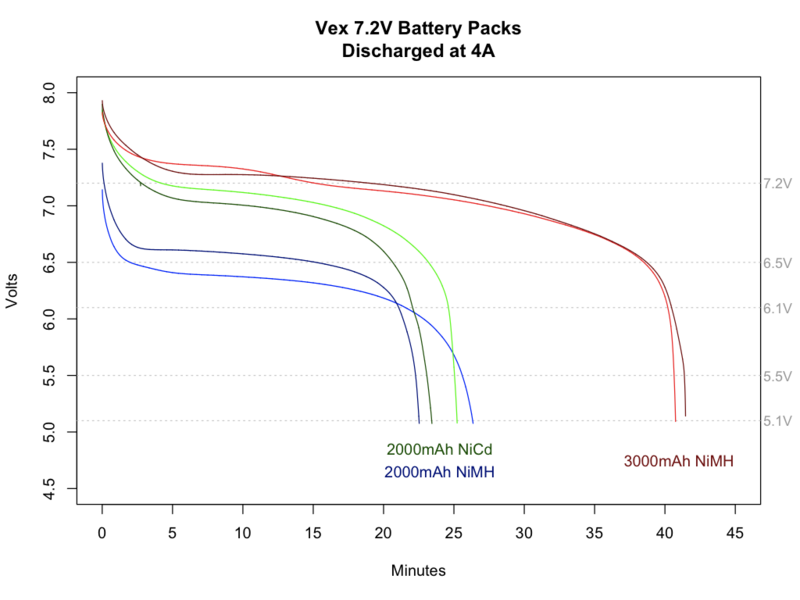
\includegraphics[width=\textwidth,height=8cm,keepaspectratio=true]{BatteryTester/DischargeGraph}
    \caption{
        The VEX battery's discharge curve over various currents, thanks to Quazar \cite{Quazar}. Notice how the voltage virtually levels out during the majority of its lifetime; This makes it difficult to get an approximate percent throughout the entire lifetime of the battery with just voltage without using integration.
    }
\end{figure}

To try to at least an accurate reading without calculus, I made a discharge curve using 2-4 motors as the load over time and made it a function of voltage (This was inspired by how another team, Renegade Robotics \cite{RenegadeRobotics}, does it). With this function, I was able to determine the approximate remaining battery capacity of our battery by measuring it's unloaded voltage, thus finishing the software aspect of this project.

\begin{figure}[h]
    \centering
    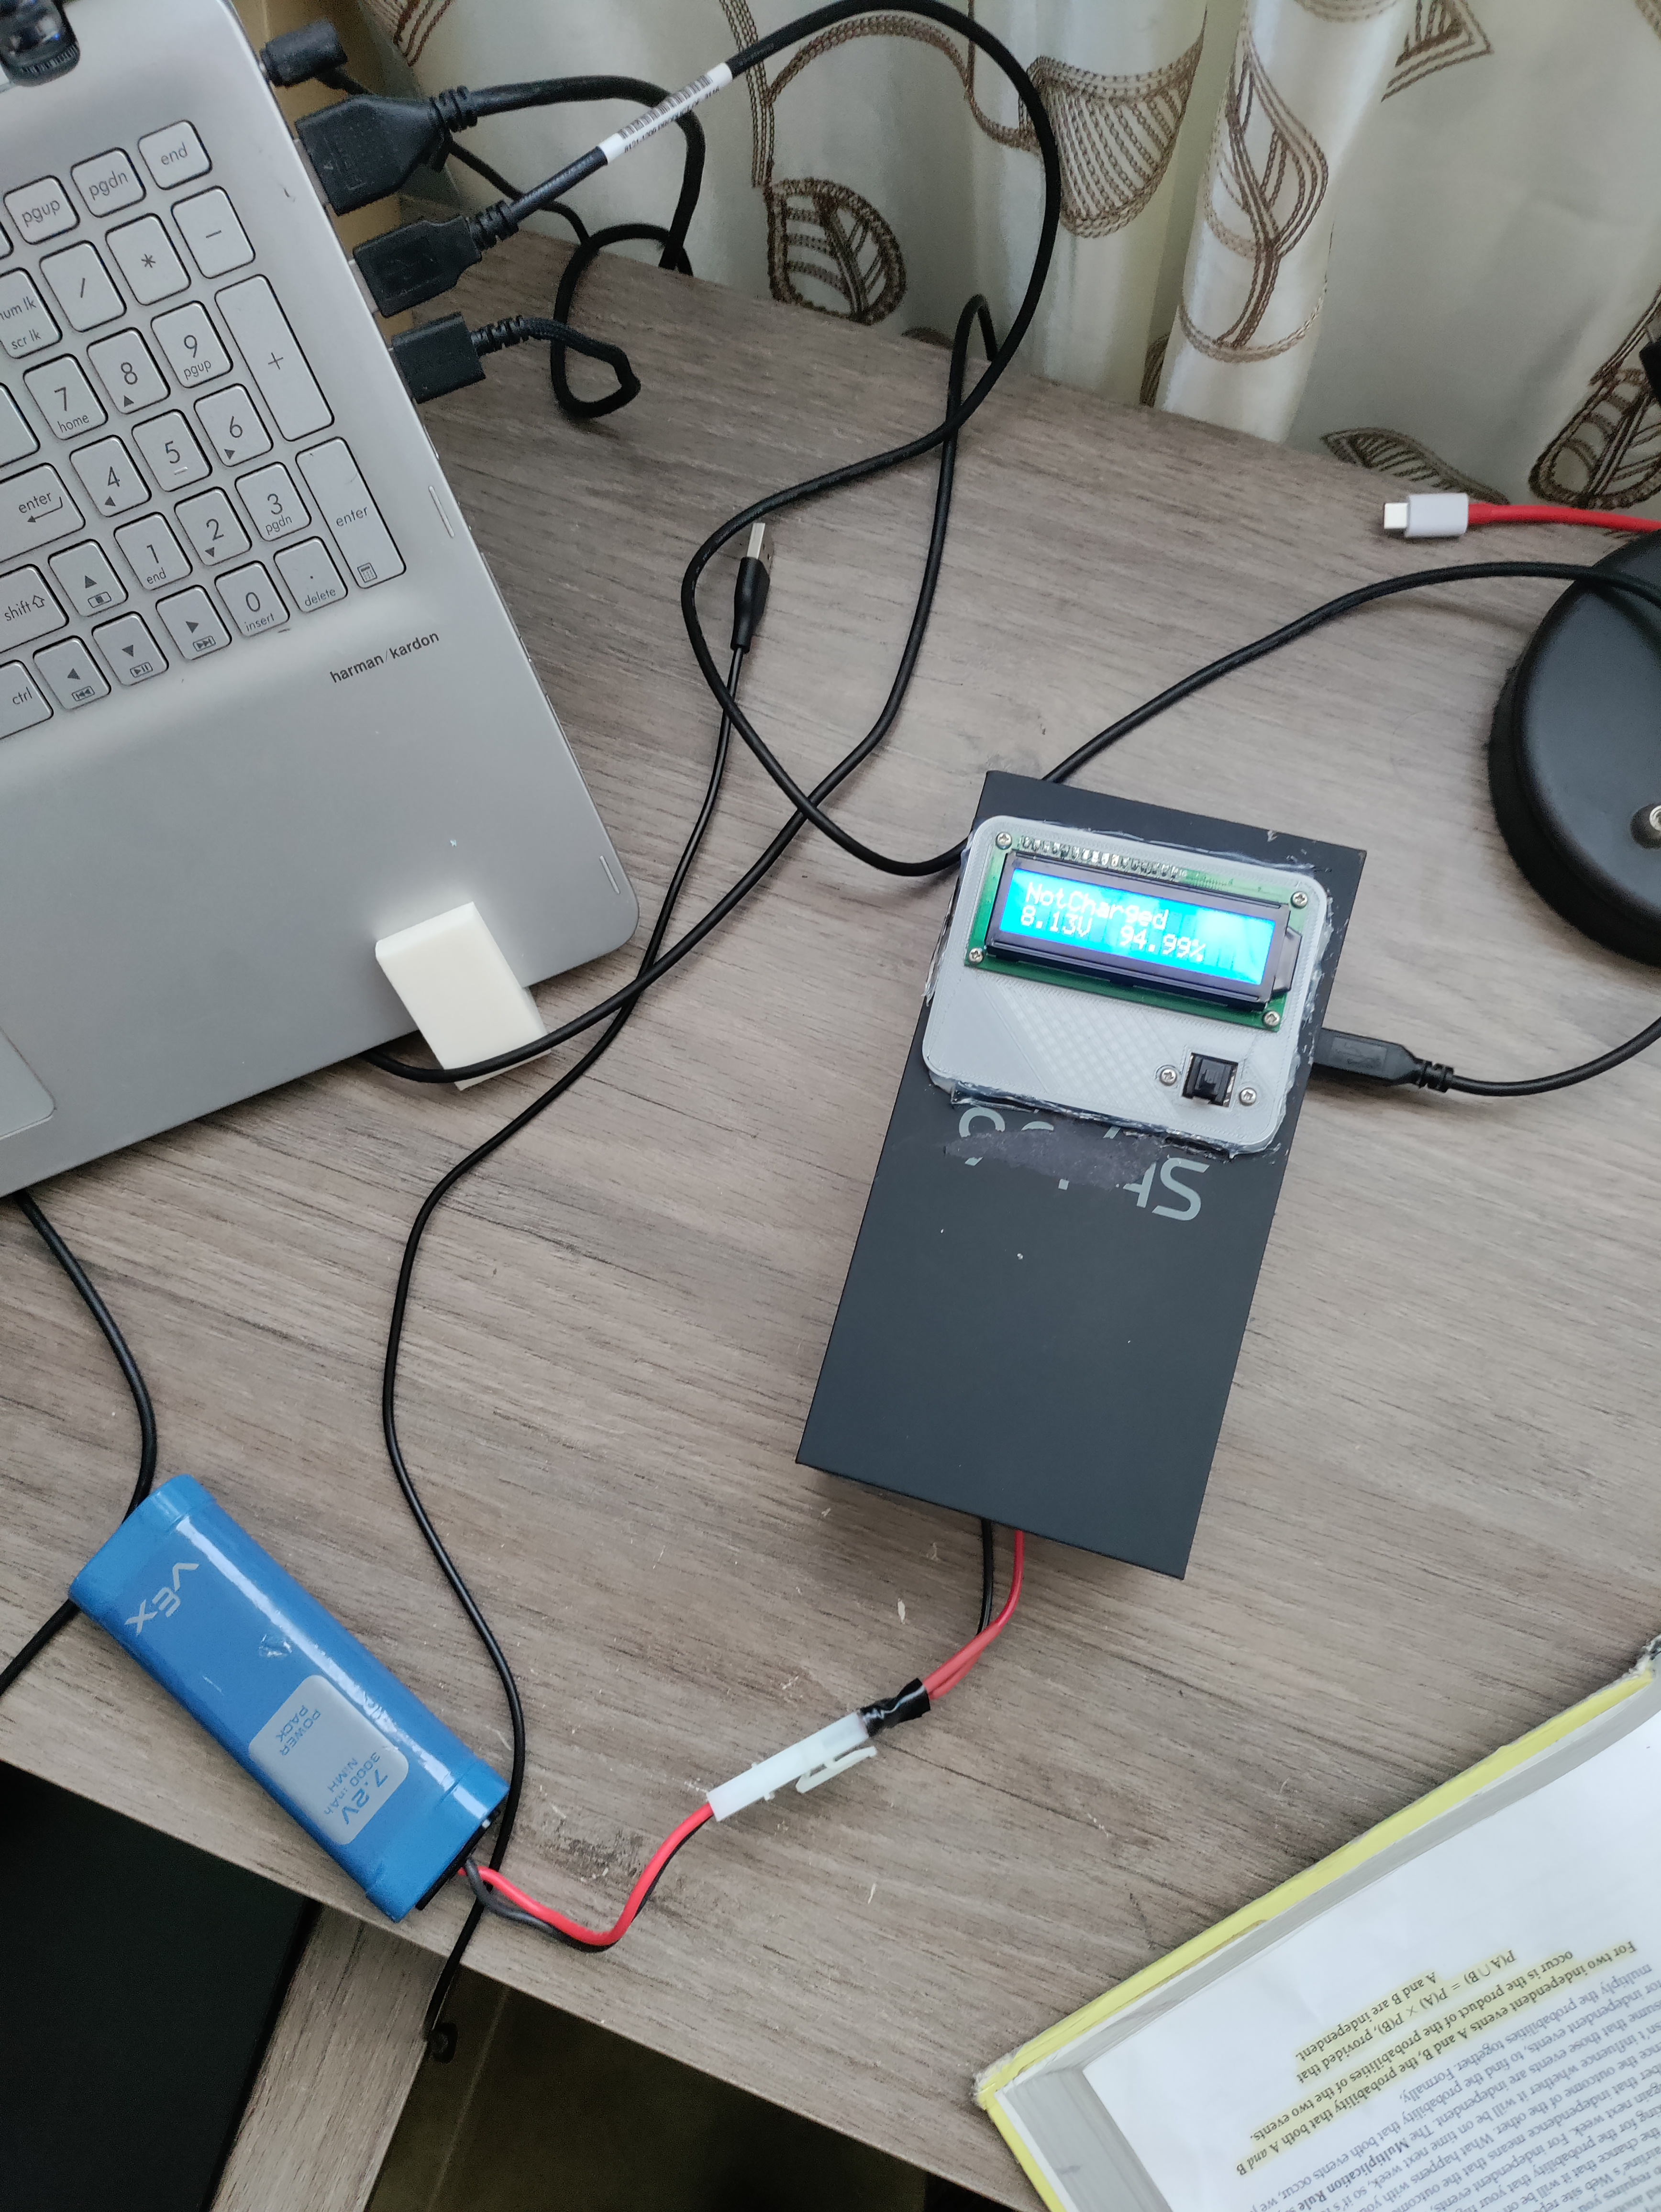
\includegraphics[width=\textwidth,height=7cm,keepaspectratio=true]{BatteryTester/BatteryTesterPortable}
    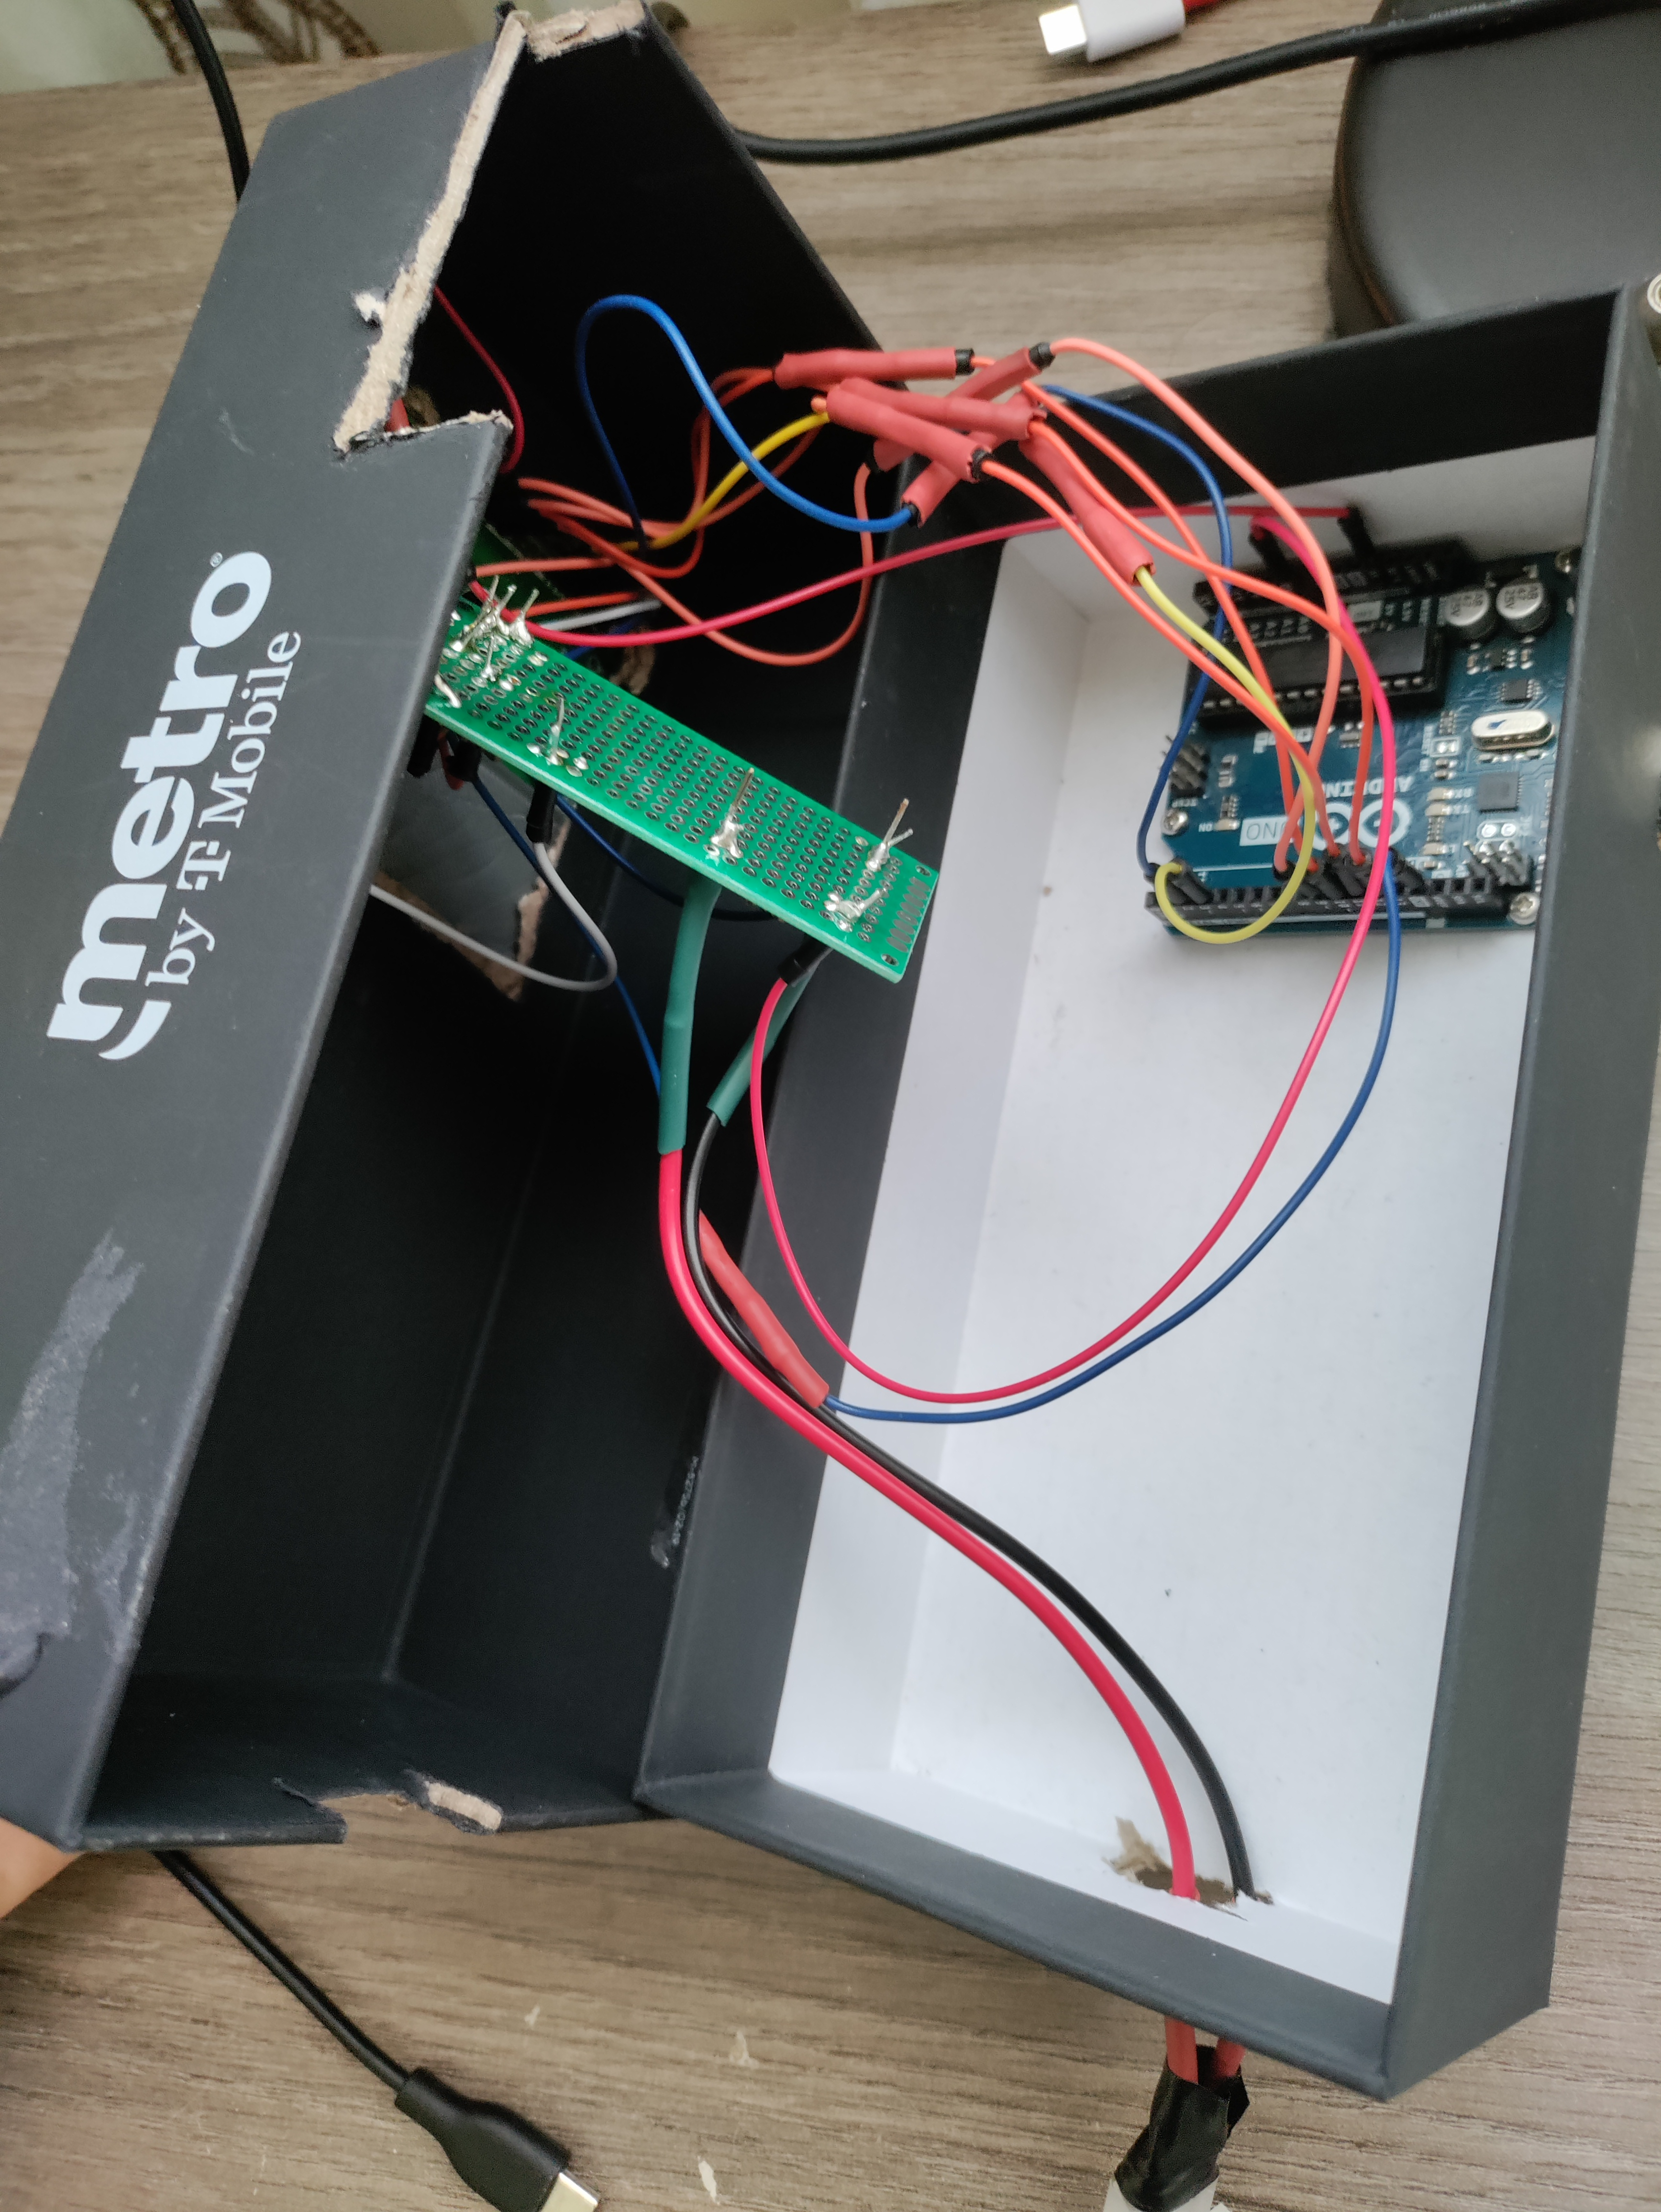
\includegraphics[width=\textwidth,height=7cm,keepaspectratio=true]{BatteryTester/BatteryTesterPortInside}
    \caption{
    The portable version of this project crammed into an old phone box. A blank PCB was used instead of a breadboard in this version to prevent the battery from accidentally shorting itself in the case it were ever dropped. The button is used to toggle the backlight to control power consumption, so that it can be powered by a mobile battery efficiently.
    }
\end{figure}

After that, I crammed the electronics into an old phone box, used leftover screws and nuts to secure its components, and called it a day.
